\section{Project Summary}
The project involves the development and implementation of an advanced book review website designed to provide users with insightful reviews and tailored book recommendations. This platform integrates sentiment analysis to evaluate and categorize user reviews, offering a nuanced understanding of reader sentiments. Additionally, it employs a recommendation engine to suggest books based on individual preferences and past interactions.
\section{Objective}
\begin{enumerate}
	\item Sentiment Analysis Integration: Implement natural language processing (NLP) techniques to analyze user reviews. This feature will categorize reviews into positive, negative, or neutral sentiments, allowing users to quickly gauge the overall reception of a book.
	\item Personalized Book Recommendations: Develop a recommendation system that leverages user data, including reading history, review sentiments, and preferences, to suggest books that align with individual tastes. This system aims to enhance user engagement by providing relevant and personalized book suggestions.
	\item User Experience Enhancement: Create an intuitive and user-friendly interface that allows users to easily navigate the sentiment analysis results and receive accurate book recommendations. The platform will also facilitate interaction through features like user profiles, book ratings, and review comments.
\end{enumerate} 
\section{Project Scope}
The scope of this project is to develop a dynamic book reviewing website that integrates advanced sentiment analysis and a personalized recommendation system. The primary goal is to create a platform where users can post and browse book reviews, while leveraging sentiment analysis to provide insights into the emotional tone of reviews. This system will analyze user reviews to categorize them as positive, negative, or neutral, and use this data to generate more accurate book recommendations tailored to individual preferences. The project will cover the design and development of the website's user interface, implementation of sentiment analysis algorithms, and the development of a recommendation engine that uses machine learning techniques to suggest books based on user interactions and review patterns. The scope also includes setting up a database for managing book information and user reviews, as well as ensuring the website is scalable and secure. Excluded from this scope are major enhancements to the website's infrastructure, such as integrating with third-party book databases or advanced user analytics tools beyond the initial requirements. The project is anticipated to be completed within a nine-month period, with milestones including website design approval, completion of sentiment analysis and recommendation features, and final user testing and launch.

\section{Key Features}
\begin{itemize}
	\item Sentiment Analysis Engine: Uses machine learning algorithms to analyze the text of user reviews and assign sentiment scores, offering users a quick summary of the book's reception.
	\item Recommendation Algorithm: Utilizes collaborative filtering, content-based filtering, and hybrid approaches to provide personalized book recommendations based on user behavior and preferences.
	\item User Profiles: Allows users to create and manage profiles, track their reading history, and receive customized book suggestions.
	\item Review System: Provides a platform for users to submit and view book reviews, along with sentiment analysis summaries.
	\item Interactive Dashboard: Features an easy-to-navigate interface for users to access sentiment analysis results, book recommendations, and manage their profiles.

\end{itemize}

\section{Methodology}
\subsection{Tools}
The project utilizes Django as the backend framework to handle server-side logic and data management. For the frontend, Bootstrap is employed as the CSS framework to ensure a responsive and visually appealing user interface. Sqlite serves as the database to store and manage book reviews, user data, and recommendation metrics. Version control is managed using Git, with repositories hosted on GitHub to track changes and facilitate collaboration.

\subsection{Data Collection \& Preparation} 
The dataset contains key information about books, including fields such as ID, title, description, authors, image, publisher, publication date, and categories. Below is a general explanation of each attribute:
\begin{enumerate}
	\item ID: A unique identifier for each book entry. This helps in managing and retrieving book data efficiently within a larger system.
	\item Title: The name of the book. It gives a clear idea of the subject or theme of the book and is used for identifying and searching books within the dataset.
	\item Description: A brief summary that provides insight into the book’s content, themes, or focus. It helps users quickly understand what the book is about.
	\item Authors: The names of the individuals who wrote the book. This field is important for users interested in finding works by specific authors.
	\item Image: A link to the cover image of the book. Including an image adds a visual reference, which is useful for enhancing the presentation of books in online platforms or catalogs.
	\item Publisher: The entity responsible for publishing the book. It helps users who may be interested in books from certain publishers or who are exploring books based on publication sources.
	\item Published Date: The date when the book was officially released. This information is important for users seeking books from a particular time period or understanding the historical context of a work.
	\item Categories: The genre or subject area the book belongs to. This allows for easier classification and filtering, helping users search for books within specific genres or areas of interest.
\end{enumerate}

This dataset\footnote{Bakhet, M. (2023). Amazon Books Review [Data set]. Kaggle. https://www.kaggle.com/datasets/mohamedbakhet/amazon-books-review} provides essential details that can be used to create a book catalog, build a recommendation system, or enhance user experience on a book review platform. Each field plays a key role in organizing and presenting book information effectively.

The database relationships (see fig.\ref{fig:database}) are primarily designed to represent books, authors, categories, reviews, and sentiments in a book review platform. The Book model serves as the central entity, connected to other models through various relationships.

The Author model has a many-to-many relationship with the Book model through the authors field. This means that a single book can have multiple authors, and an author can be associated with multiple books.

Similarly, the Category model also has a many-to-many relationship with the Book model via the categories field. A book can belong to multiple categories (e.g., Fiction, Science Fiction, Biography), and each category can contain multiple books.

The Review model has a foreign key relationship with both the Book and the CustomUser models. Each review is associated with a specific book and user, meaning that a user can leave multiple reviews for different books, and a book can have multiple reviews from different users.

Additionally, the Review model has a foreign key relationship with the Sentiment model, which stores the sentiment analysis results. The sentiment field is nullable, indicating that it is optional for a review. The sentiment is assigned dynamically after the review is saved using sentiment analysis, such as TextBlob. The sentiment is either "very negative," "negative," "neutral," "positive," or "very positive," and is mapped to an integer value through the Sentiment model.
\begin{figure}[h!]
	\begin{center}
		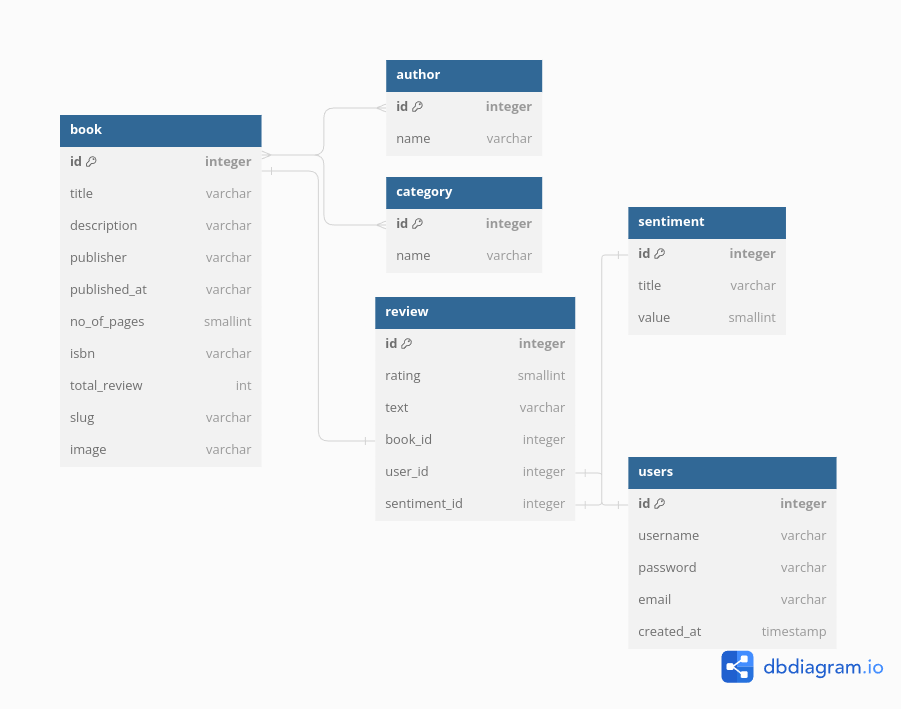
\includegraphics[width=.6\textwidth]{schema.png}
	\end{center}
	\caption{Schema Diagram for the Database}\label{fig:database}
\end{figure}

\subsection{Sentiment Analysis}
Some common libraries used for sentiment analysis are 
NLTK, TextBlob, spaCy, RoBERTa etc. 
In this project, I chose to use the \textbf{TextBlob} library because
the project was intended to be a prototype and TextBlob has a smaller
size and acceptable results compared to other libraries.
Although, RoBERTa and spaCy have more accurate results but their size
is not suitable for small scale server projects. They require much
processing power.
\begin{figure}[h]
	\begin{center}
		
\includegraphics[width=.5\textwidth]{textblob.png}
	\end{center}
	\caption{TextBlob library logo}\label{fig: Textblob library logo}
\end{figure}


\section{Images}
\movie[externalviewer]{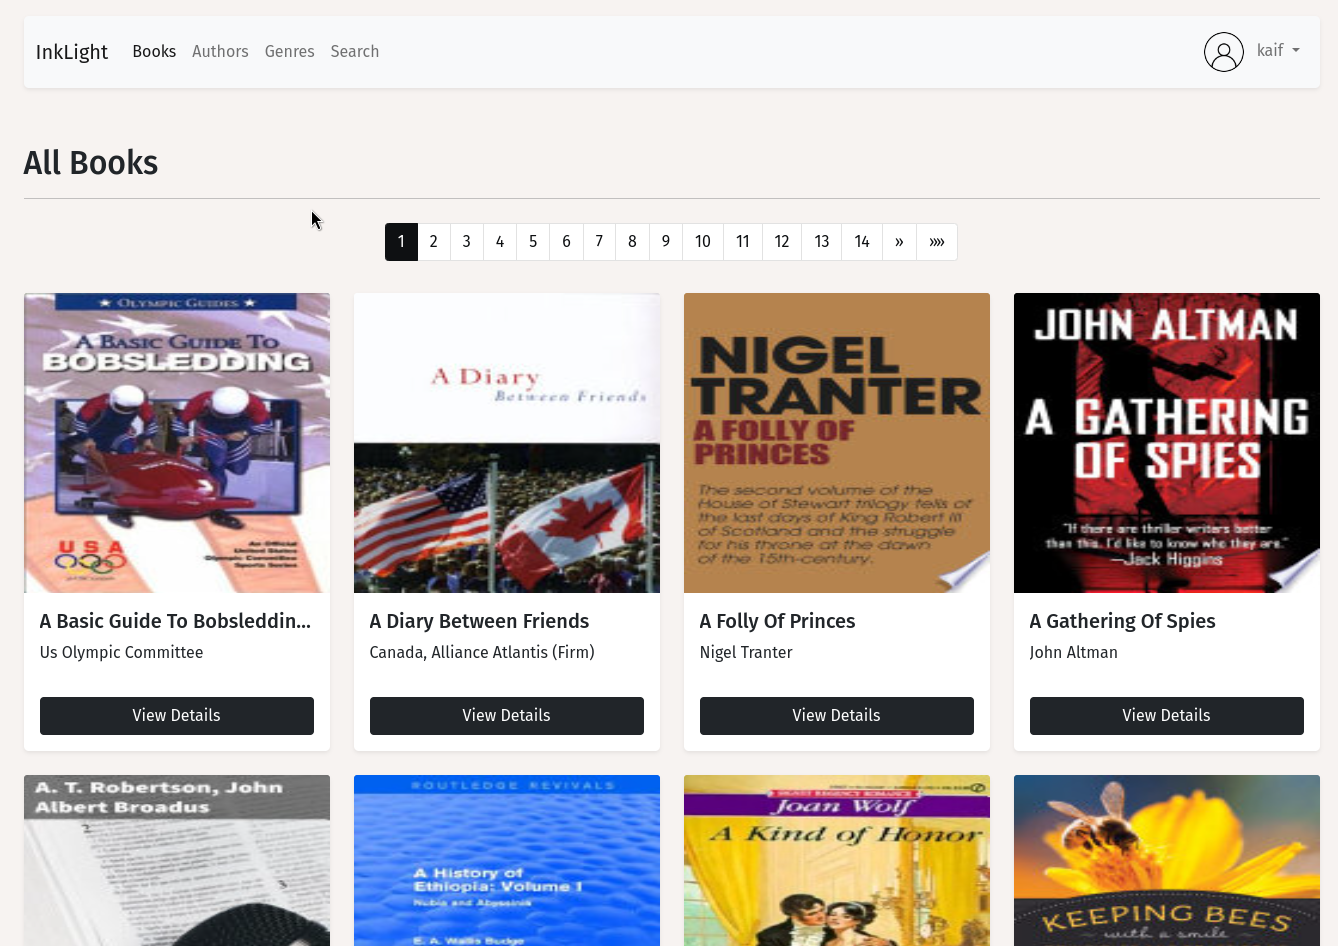
\includegraphics[width=\textwidth,keepaspectratio]{video.png}}{video.mp4}

\section{Future Works}

\subsection{Improving Sentiment Analysis}
The current sentiment analysis uses TextBlob, which is suitable for basic analysis but may not capture the full range of emotions in book reviews. To improve accuracy, we could introduce more advanced models like BERT or GPT, which are better at understanding complex sentences and context. Additionally, training these models with specific book review data would help them better recognize the unique tone and style of literary reviews. Expanding the analysis to cover more dimensions of sentiment, such as emotional tone and writing style, would provide a more detailed understanding of user reviews.

\subsection{Better Recommendation System}
The recommendation system can be enhanced by using more personalized approaches. Collaborative filtering, which suggests books based on the preferences of similar users, could improve the accuracy of recommendations. We could also implement content-based filtering, which analyzes the book's themes and genres to make suggestions based on a user’s reading history. Combining both methods into a hybrid system would offer a more balanced and accurate set of recommendations. Machine learning techniques can also be used to continually refine suggestions based on a user’s evolving preferences.

\subsection{Bangla Language NLP}
Expanding the platform to include Bangla (Bengali) support would allow us to reach a larger audience. For sentiment analysis in Bangla, models like Bangla BERT can be fine-tuned to understand the nuances of the language. Handling specific challenges like the complex structure of Bangla words is important for accurate analysis. Adding multilingual support for both English and Bangla reviews would create a more inclusive platform, while a separate recommendation engine for Bangla literature would cater to users interested in Bangla books. This would enhance the platform’s appeal to Bangla-speaking readers.
\section{Conclusion}
Project Codebase:
\url{https://github.com/ahmed-kaif/inklight}
